\chapter{Contact Graph Routingによる運用とその研究}
\label{chap:DTNにおけるルーティングの研究と課題}

\ref{subsection:ネットワークトポロジーの変動と間欠的接続}項で述べた通り、
宇宙のネットワークにおけるノードの多くは衛星であり、その位置は常に変動する。
そのためノード間の通信は特定の時間にのみ可能なものであり、
この間欠的なリンクを順次利用して転送しEnd-to-Endのデータグラムの転送を行う必要がある。
DTNでは、特定の2つのノード間の通信が可能なこの時間やタイミングをContactと呼び、
軌道計算などにより事前に計画されたContactを次々と利用して転送を行う
Contact Graph Routing(CGR)\cite{Fraire2021}というコンセプトが構想されている。
既に述べた通り既存のDTN実装は複数あるが、これらのDTN実装における
ルーティング手法でも主にCGRが用いられ、宇宙データ通信システムに関わる国際標準化検討委員会である
宇宙データシステム諮問委員会(CCSDS : Consultative Committee 
for Space Data System)ではSCHEDULE-AWARE BUNDLE ROUTING
\cite{schedule_aware_bundle_routing}として標準化されている。
DTNでCGRを用いたルーティングを運用する場合、その運用プロセスは以下の3つの段階に大別できる。
1つ目の段階は運用計画の決定、2つ目はルート決定、3つ目は実際のバンドルの転送である。
本章ではそれぞれの段階ごとにDTNにおけるCGRとその研究について分類し、現状の課題について説明する。
\section{運用計画の決定}
\label{section:運用計画の決定}
1つ目の段階では、ミッションコントロールなどを担う地上局など(以後、マスターノードとする)が、
各ノードの軌道計算やその他の情報に基づいてContact Planを作成する。
宇宙におけるノードの物理的な軌道は計算により予測可能であり、
2ノード間のContactも事前に計算することが可能である。 
CGRの例として、図\ref{fig:contact_example_topology}のようなAからDの4つのノードからなるトポロジーのDTNを考える。
マスターノードは軌道計算によるこれらのノードの位置や、搭載する機材の性能等をもとにContact Planを作成する。
Contact Planには、Contactについての記述とRangeについての記述が含まれ、
Contactについての記述では、特定の2ノードの通信機会についての通信開始・終了時間、データレートなどが記載され
(図\ref{fig:contact_example_contactplan})、Rangeについての記述では特定の2ノードの物理的な距離について記載される
(図\ref{fig:contact_example_contactrange})。
ただし\ref{subsection:通信機会の非対称性}項で述べた通り、宇宙における特定の2ノード間の通信機会は非対称であるため、
Contact Planに記載される通信機会は、特定の2ノードについての両方のリンクの通信可能機会ではなく、
片方向のリンクについての通信機会である。

\begin{figure}[tbh]
    \centering
    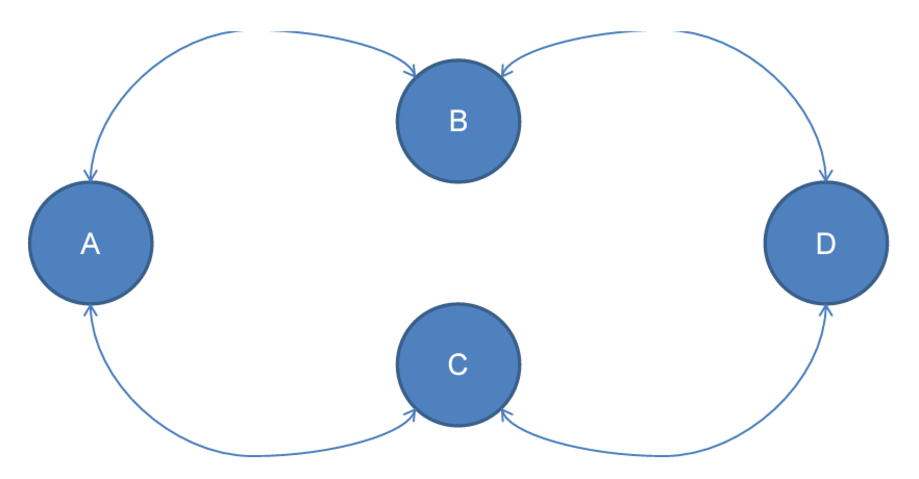
\includegraphics[width=0.5\textheight]{img/contact_example_topology.pdf}
    \caption{4つのノードからなるDTNの例}
    \label{fig:contact_example_topology}
    \begin{minipage}{\textwidth}
        \centering
        \vspace{3mm}
        参考文献\cite{schedule_aware_bundle_routing}figure3-1より引用
    \end{minipage}
\end{figure}
\begin{figure}[tbh]
    \centering
    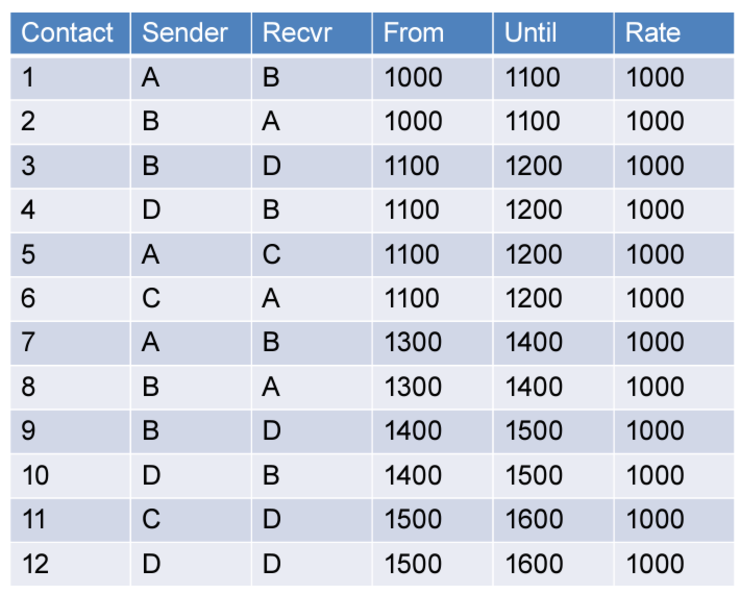
\includegraphics[width=0.5\textheight]{img/contact_example_contactplan.pdf}
    \caption{図\ref{fig:contact_example_topology}のトポロジーにおけるContact Planの例(Contactに関する表記)}
    \label{fig:contact_example_contactplan}
    \begin{minipage}{\textwidth}
        \raggedright
        \vspace{3mm}
        参考文献\cite{schedule_aware_bundle_routing}figure3-2より引用。Senderは送信元のノードの識別子、Receiverは受信元のノードの識別子、FromはContactの開始時刻、Untilは終了時刻、Rateは転送速度を示す。
    \end{minipage}
\end{figure}
\begin{figure}[tbh]
    \centering
    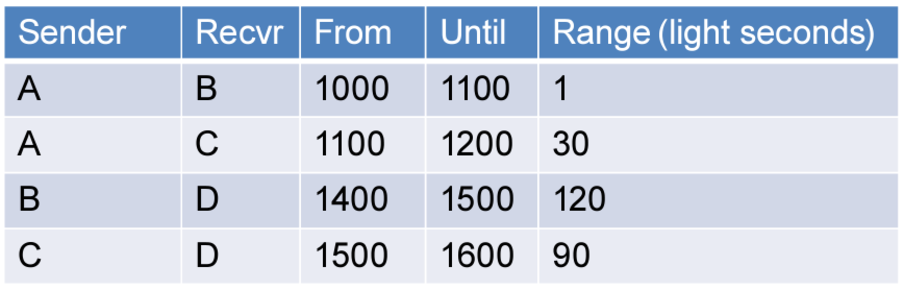
\includegraphics[width=0.5\textheight]{img/contact_example_contactrange.pdf}
    \caption{図\ref{fig:contact_example_topology}のトポロジーにおけるContact Planの例(Rangeに関する表記)}
    \label{fig:contact_example_contactrange}
    \begin{minipage}{\textwidth}
        \centering
        \vspace{3mm}
        参考文献\cite{schedule_aware_bundle_routing}figure3-3より引用。
    \end{minipage}
\end{figure}


\section{経路決定}
\label{subsection:経路決定}

\ref{section:運用計画の決定}節で決定されたContact Planは、
衛星どうしのContactを記載したものであり、実際のDTNの運用においては
Contact Planに基づいて転送すべき経路を決定する必要がある。
ノードAからノードDに向けたBundleを配送する場合、
図\ref{fig:contact_example_contactplan}
及び図\ref{fig:contact_example_contactrange}からなるContact Planに対し、
\ref{subsection:宇宙インターネットにおけるルーティングのアルゴリズム}項で述べるアルゴリズムを用いることにより
図\ref{fig:contact_example_contactgraph}のようなContact Graphを得る。
ただしContact Graphにおける頂点はDTNにおける各ノードではなく単一のContactであるため、
Contact GraphはDTNのトポロジーを示すものではなく、データ転送が可能な経路を計算するためのグラフである。

\begin{figure}[tbh]
    \centering
    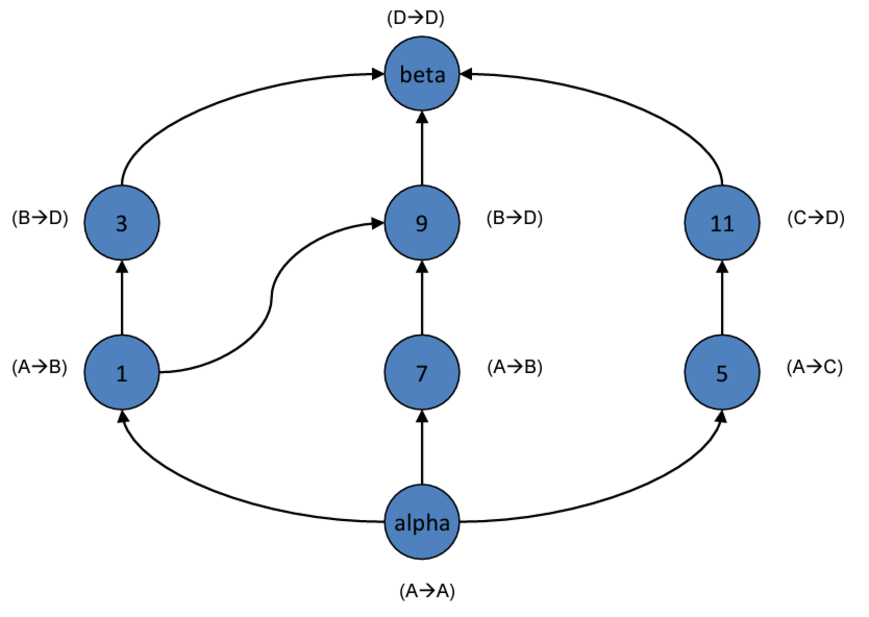
\includegraphics[width=0.5\textheight]{img/contact_example_contactgraph.pdf}
    \caption{図\ref{fig:contact_example_contactplan}及び
    図\ref{fig:contact_example_contactrange}のContact Planから計算されるContact Graphの例}
    \label{fig:contact_example_contactgraph}
    \begin{minipage}{\textwidth}
        \centering
        \vspace{3mm}
        参考文献\cite{schedule_aware_bundle_routing}figure3-4より引用。
    \end{minipage}
\end{figure}
\label{chap:related_works}


\subsection{初期のCGRにおけるルーティングのアルゴリズム}
\label{subsection:宇宙インターネットにおけるルーティングのアルゴリズム}    
CGRでは図\ref{fig:contact_example_contactgraph}に対してアルゴリズムによる
計算を行うことで最適な転送経路を決定している。
CGRは\cite{Burleigh2008}において、基本的なパラメータとコンタクトグラフの利用や、
これらを用いた転送先の近接ノードの決定などの基本的な概念が提案された。
しかしこの提案ではルーティングアルゴリズムについては、静的な経路計算に関する
アルゴリズムは規定されず、ルーティングループ防止の必要性、デフォルトルートを用いた動的
ルーティングの想定などに触れられるのみにとどまった。

\subsection{CGR-EF}
\label{subsection:CGR-EF}
Burleighは2010年に\cite{burleigh-dtnrg-cgr-01}において、
earliest forfeit time、すなわちエンドツーエンドの転送が
可能なパスにおける、そのパスの最短失効時間に注目し、その時間が短いパスから優先して
利用することで、リンク利用の効率化を図るCGR-EFを提案した。CGR-EFは
2009年10月から11月にかけて行われたディープインパクトネットワーク実験(DINET)
\cite{JPL2009}に用いられ、NASAのジェット推進研究所と宇宙船の間の約300枚の画像転送に成功した。

\subsection{ECGR}
その後Seguiらは、earliest-forfeit-timeではなくearliest-arrival-time、すなわち
エンドツーエンドの最短到達遅延を指標とするECGRを提案した\cite{6134460}。
ECGRはearliest-arrival-timeを指標とすることでより計算コストの小さい
ダイクストラアルゴリズムを用いることを可能にしており、
またルーティングループが発生しない、経路が時間とともに単調に収束することもメリットである。
これ以後、CGRにおけるアルゴリズムとしては基本的にダイクストラが用いられている。


\subsection{Yen routing algorithm}
\label{subsection:Yen routing algorithm}
Fraireらはルーティングテーブルの管理手法について研究を行い、
これに基づき現状のCGRは基本的にYen Routing Algorithmを用いている。\cite{FRAIRE2018}

\subsection{CGRに代替するアルゴリズム}
\label{subsection:CGRに代替するアルゴリズムの研究}
Efficient Contact Graph Routing Algorithms for Unicast and Multicast Bundles
\cite{DeJonckere2019}

\section{バンドルの転送}
\label{section:バンドルの転送}


\section{Contact Planの更新}
\label{sec:ContactPlanの更新}
このようにCGRのアルゴリズム・パラメータについての研究は多く行われているが、
これらはContact Planをもとに経路を計算手法の研究であり、
経路計算を行いたいノードにおいてそもそもContact Planが存在していることが前提となる。
そのため、Contact Planをノードに配送する手法が必要となるが、
Contact Planはその性質上、更新が必要であり、定期更新と臨時更新に分けて考えることができる。

\subsection{Contact Planの定期更新}
\label{sec:ContactPlanの定期更新}
Contact Planは有限時間内でのContactについて記述したものであり、
その時間以降のContact Planに関しては定期的に更新する必要がある。
ただし、Contact Planに記載されるノードの全てが周期的な運動のみを行う場合には
Contact Planを繰り返し使える可能性がある。

\subsection{Contact Plan の臨時更新}
\label{sec:ContactPlanの臨時更新}
ここでは故障時などのContact Planの臨時更新について述べる。
先行研究として\cite{Bezirgiannidis2013}を用いる。

\section{問題提起}
\label{sec:ContactPlanの臨時更新の課題}
\ref{sec:ContactPlanの臨時更新}で述べたように、想定されたContactに失敗が発生した場合、
その情報をDTNの他のノードに拡散しContact Planを更新することで、
DTNの各ノードはその時点におけるネットワークの最新のトポロジーと一致するContact Planを
保持することができ、これによりより適する経路がある場合これを選択することが可能になる。
しかし実際にリンク障害などが発生した場合、DTNの各ノードにその情報の拡散が完了する時間は、
拡散を開始するノードからCGRによってその情報を格納したバンドルが到達する時間によって決まる。
そのため天体間にまたがるDTNを運用しており、それらの全てノードに通知を行うことを想定した場合、
\ref{subsection:大きな遅延のある通信環境}で述べた天体間の遅延と、
さらにその天体内でのContact Planに応じた時間分、障害情報の拡散の完了までには大きな時間を要する。

そのためContact Planの臨時更新においては、
必要なノードにのみ効率よくその情報を拡散し遅延を抑えることを達成することが求められる。